\documentclass[UTF8,a4paper,12pt,openany]{ctexbook}

\newcommand{\ReportTitle}{具身智能行业和技术发展调研报告}
\newcommand{\ReportVersion}{v0.2}
\newcommand{\ReportAuthor}{个人学习与研究用途}

\newcommand{\ReportBibStyle}{gb7714-2015}
\usepackage{geometry}
\geometry{a4paper, left=28mm, right=28mm, top=25mm, bottom=25mm, headheight=15pt}

\usepackage{amsmath,amssymb,mathtools}
\usepackage{graphicx}
\usepackage{booktabs}
\usepackage{array}
\usepackage{longtable}
\usepackage{tabularx}
\usepackage{xltabular}
\usepackage{adjustbox}
\usepackage{enumitem}
\usepackage{float}
\usepackage{xcolor}
\usepackage{listings}
\usepackage{caption}
\usepackage{newunicodechar}
\usepackage{hyperref}
\usepackage{url}
\providecommand{\ReportBibStyle}{authoryear}
\usepackage[backend=biber,style=\ReportBibStyle]{biblatex}
\addbibresource{references/references.bib}
\AtBeginBibliography{\raggedright}

\setCJKmainfont{FangSong}[AutoFakeBold=0.2,AutoFakeSlant=0.15]
\setCJKsansfont{SimHei}
\setCJKmonofont{FangSong}
\setmainfont{FangSong}[AutoFakeBold=0.2,AutoFakeSlant=0.15]
\setsansfont{SimHei}
\setmonofont{FangSong}
\newunicodechar{•}{\ensuremath{\bullet}}

\hypersetup{
  colorlinks=true,
  linkcolor=black,
  urlcolor=blue,
  citecolor=black,
  pdftitle={\ReportTitle-\ReportVersion},
  pdfauthor={\ReportAuthor}
}

\setlist[itemize]{leftmargin=2em, itemsep=2pt, topsep=4pt}
\setlist[enumerate]{leftmargin=2em, itemsep=2pt, topsep=4pt}
\renewcommand{\labelitemi}{$\bullet$}
\renewcommand{\labelitemii}{$\circ$}
\setlength{\parindent}{2em}
\setlength{\parskip}{0.35em}
\setlength{\emergencystretch}{3em}
\raggedbottom
\linespread{1.25}

% The 27 report parts are the page-level divisions. Numeric chapters and
% subsections remain in the current page flow unless natural pagination occurs.
\newcommand{\reportpart}[1]{%
  \clearpage
  \phantomsection
  \noindent{\fontsize{18pt}{24pt}\selectfont\bfseries #1\par}%
  \medskip
}

\lstset{
  basicstyle=\small\ttfamily,
  breaklines=true,
  breakatwhitespace=false,
  columns=fullflexible,
  frame=single,
  keepspaces=true,
  showstringspaces=false,
  numbers=left,
  numbersep=8pt,
  xleftmargin=2em,
  literate={π}{{$\pi$}}1 {Δ}{{$\Delta$}}1 {≈}{{$\approx$}}1 {×}{{$\times$}}1
}

\newcolumntype{Y}{>{\raggedright\arraybackslash}X}
\graphicspath{{figures/}{../../../../assets/images/}{../../../../assets/diagrams/}}

\newcommand{\evidencefact}[1]{\par\noindent\textbf{证据事实：}#1\par}
\newcommand{\authorjudgement}[1]{\par\noindent\colorbox{black!6}{\parbox{0.94\linewidth}{\textbf{综述判断：}#1}}\par}
\newcommand{\sourceanchor}[1]{\par\small\noindent\textit{源码锚点：}#1\par\normalsize}

\addbibresource{references/pilot-v0.3.bib}

\title{\ReportTitle\ v0.3 写作标准双试点}
\author{\ReportAuthor}
\date{2026-07-13}

\begin{document}
\frontmatter
\maketitle
\chapter*{试点说明}
本文件只装配已获批准的第 6 章和第 23 章，用于验证 v0.3 的教材型综述写法。它不替代全书 \texttt{main.tex}，也不把尚未重写的 v0.2 章节标记为 v0.3 完成稿。
\tableofcontents

\mainmatter
\chapter{动力学、接触与柔顺控制}
\label{chap:dynamics-contact-compliance}

\section{学习目标、前置知识与问题边界}

读完本章，读者应能从机械臂的能量出发写出关节空间动力学，解释接触互补条件和摩擦锥的物理意义，推导任务空间阻抗控制律，并把一项柔顺插装任务拆成观测、控制、阈值与恢复四个相互独立的设计问题。前置知识是第 5 章中的齐次变换、雅可比矩阵和速度映射。本章不把“接触成功”归因于某一个控制器：孔位估计错误、工件公差、末端标定、传感延迟和恢复策略都可能决定结果。

刚性自由空间轨迹跟踪要求机器人逼近给定位置；接触操作则要求机器人在几何不确定时限制交互力。二者的差别不是“是否加一个力传感器”，而是受控对象从位姿误差扩展为机器人与环境组成的耦合动力系统。Hogan 的阻抗控制把目标写成力与运动之间的动态关系，而不是把位置或力之一孤立地设为唯一输出\cite{hogan1985impedance}；Khatib 的操作空间公式进一步给出了任务坐标中的惯量和力映射\cite{khatib1987operational}。

\section{从能量到关节空间动力学}

设 $q\in\mathbb{R}^{n}$ 为关节位置，$\dot q$、$\ddot q$ 分别为速度和加速度。机械臂的动能和势能写为
\begin{equation}
T(q,\dot q)=\frac{1}{2}\dot q^\top M(q)\dot q,\qquad V(q),
\end{equation}
其中 $M(q)$ 是对称正定惯量矩阵。对拉格朗日量 $L=T-V$ 应用 Euler--Lagrange 方程，可得
\begin{equation}
M(q)\ddot q+C(q,\dot q)\dot q+g(q)+\tau_f
=\tau+J_c(q)^\top\lambda .
\label{eq:joint-dynamics}
\end{equation}
$\tau$ 是执行器力矩，$g(q)=\partial V/\partial q$，$\tau_f$ 汇集关节摩擦等未建模项，$J_c^\top\lambda$ 把接触点的广义力映射到关节空间。$C$ 的矩阵表示不是唯一的，但应满足 $\dot M-2C$ 反对称；该性质使无耗散、无外力系统的能量变化与输入功率一致，是许多稳定性推导的关键\cite{featherstone2008rigid,lynch2017modern}。

式中各项的量纲都必须是力矩：$M\ddot q$ 是产生关节加速度所需的惯性力矩，$C\dot q$ 汇集由速度引起的科氏与离心力矩，$g$ 抵消重力，$\tau_f$ 表示摩擦和传动损失。接触项来自虚功等价：接触点虚位移满足 $\delta x_c=J_c\delta q$，外力做功
\begin{equation}
\delta W=\lambda^\top\delta x_c
=\lambda^\top J_c\delta q
=(J_c^\top\lambda)^\top\delta q,
\end{equation}
所以与接触力等价的关节广义力必为 $J_c^\top\lambda$。这也解释了为什么末端力传感器读数不能直接加到关节力矩上：必须先统一坐标系、符号和力矩参考点，再乘雅可比转置。

反对称性质还给出一个有用的能量检查。令机械能 $E=T+V$，把式\eqref{eq:joint-dynamics}左乘 $\dot q^\top$，利用 $\dot q^\top(\dot M-2C)\dot q=0$，可得
\begin{equation}
\dot E=\dot q^\top\tau+(J_c\dot q)^\top\lambda-\dot q^\top\tau_f.
\label{eq:robot-power-balance}
\end{equation}
右侧依次是执行器输入功率、环境通过接触注入的功率和摩擦耗散。仿真器若在无输入、无接触、无摩擦时让 $E$ 持续增长，通常意味着积分器、$C$ 的实现或坐标变换存在错误。

式\eqref{eq:joint-dynamics}对应三类计算。逆动力学已知 $(q,\dot q,\ddot q)$ 求 $\tau$，用于前馈补偿；正动力学已知 $(q,\dot q,\tau)$ 求 $\ddot q$，用于仿真和预测；参数辨识则由多段运动和力矩数据估计质量、质心、惯量及摩擦参数。三者不能混用：一个能在低速轨迹上拟合力矩的模型，未必能预测碰撞冲量，因为后者还依赖接触几何、恢复系数和采样时间。

\subsection{二连杆算例：耦合项如何进入控制}

对平面二连杆，若忽略摩擦，惯量矩阵可写成
\begin{equation}
M(q)=\begin{bmatrix}
a+2b\cos q_2 & d+b\cos q_2\\
d+b\cos q_2 & d
\end{bmatrix},
\end{equation}
其中 $a,d$ 由连杆质量、长度和转动惯量组成，$b=m_2l_1l_{c2}$。取 $a=3.2$、$b=0.6$、$d=0.5\ \mathrm{kg\,m^2}$，当 $q_2=0$ 时
$M=\left[\begin{smallmatrix}4.4&1.1\\1.1&0.5\end{smallmatrix}\right]$；当 $q_2=\pi/2$ 时变为
$M=\left[\begin{smallmatrix}3.2&0.5\\0.5&0.5\end{smallmatrix}\right]$。同一关节加速度命令在不同姿态需要不同力矩。只使用常数增益而没有模型补偿时，姿态改变会表现为响应速度和超调变化；这不是神经网络特有的“分布偏移”，而是机械系统本身的构型依赖。

例如忽略 $C$ 与 $g$，要求 $\ddot q=[1,0]^\top\ \mathrm{rad/s^2}$，伸直姿态需要惯性力矩 $[4.4,1.1]^\top\ \mathrm{N\,m}$，而 $q_2=\pi/2$ 时只需 $[3.2,0.5]^\top\ \mathrm{N\,m}$。第二关节虽然没有加速度，仍因非对角项收到 $1.1$ 或 $0.5\ \mathrm{N\,m}$；这就是动态耦合。真实逆动力学还必须把 $C\dot q$、$g$ 和期望接触力加入，算例只隔离惯量项。

\section{单边接触、摩擦与混合动力学}

令 $\phi(q)$ 为两物体的法向间隙，$\phi>0$ 表示分离，$\phi=0$ 表示接触。刚性、不可穿透接触的理想化法向条件是
\begin{equation}
0\leq \lambda_n\ \perp\ \phi(q)\geq 0,
\label{eq:complementarity}
\end{equation}
即 $\lambda_n\geq0$、$\phi\geq0$ 且 $\lambda_n\phi=0$。它排除了“尚未接触却产生推力”和“接触时仍相互穿透”两种状态。切向力满足库仑摩擦锥
\begin{equation}
\|\lambda_t\|_2\leq \mu\lambda_n.
\label{eq:friction-cone}
\end{equation}
严格位于锥内可以粘着；达到边界后可能滑动，方向与相对切向速度相反。数值算法常把圆锥多面体化以转成线性互补问题，但边数越少，摩擦方向误差越大。

互补式只允许两种法向模式：分离时 $\phi>0,\lambda_n=0$；承压接触时 $\phi=0,\lambda_n\ge0$。$\phi=0,\lambda_n=0$ 是即将建立或断开的边界状态，而 $\phi>0,\lambda_n>0$ 和 $\phi<0$ 都不合法。摩擦锥还要结合切向速度理解：$\|\lambda_t\|<\mu\lambda_n$ 时，约束求解器可以选择足以阻止滑动的切向力；到锥面时，若仍有相对运动，摩擦方向与切向速度相反。式\eqref{eq:friction-cone}给的是可行集合，不是独立计算 $\lambda_t$ 的控制律。

\begin{figure}[H]
\centering
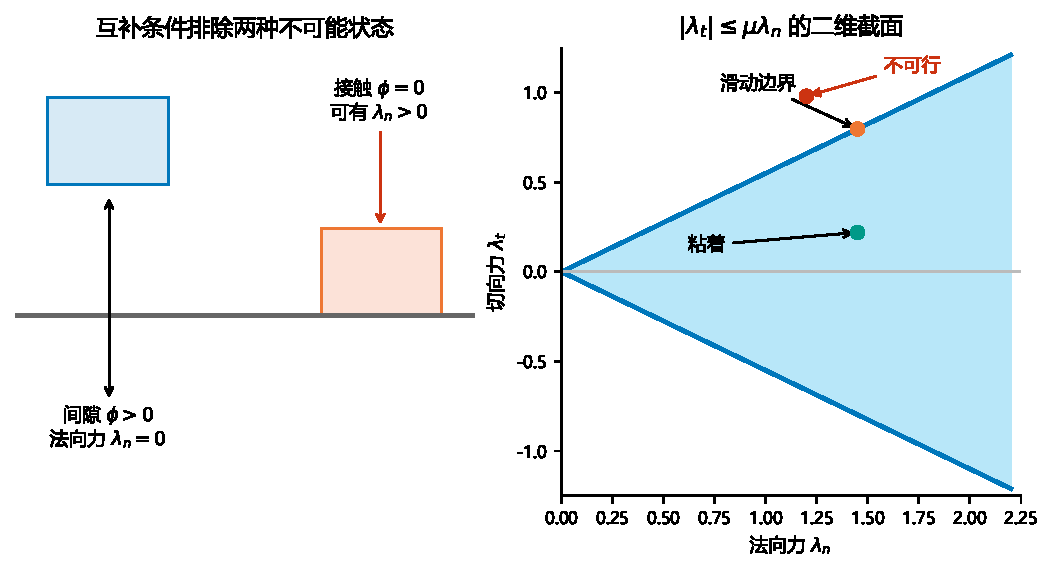
\includegraphics[width=\textwidth]{v0.3-06-接触互补与摩擦锥.pdf}
\caption{法向互补的合法/非法状态与库仑摩擦锥截面。作者依据刚性接触模型绘制；图为概念解释，不是实验数据\cite{featherstone2008rigid,lynch2017modern}。}
\label{fig:contact-complementarity-friction}
\end{figure}

接触建立或断开会改变约束集合，碰撞还会使速度发生跃迁。因此接触操作是混合系统：连续阶段用式\eqref{eq:joint-dynamics}演化，离散事件更新接触模式或施加冲量。柔顺材料和有限采样控制器常用罚函数 $\lambda_n=k_p[-\phi]_++d_p[-\dot\phi]_+$ 近似接触；它容易实现，却把允许穿透量、刚度和积分步长绑定在一起。减小步长并不自动消除模型偏差，增大刚度也可能造成数值发散。

\begin{table}[H]
\centering
\caption{接触建模选择及其代价}
\label{tab:contact-models}
\begin{tabularx}{\textwidth}{p{0.18\textwidth}YYY}
\toprule
方法 & 主要变量 & 优点 & 典型失效\\
\midrule
刚性互补 & 间隙、接触力/冲量 & 不允许静态穿透，接触逻辑明确 & 求解不光滑，多接触时计算昂贵\\
罚函数 & 穿透量、相对速度 & 易并入常微分方程和自动微分 & 刚度与步长耦合，参数缺乏真实对应\\
可变形接触 & 形变场或局部材料参数 & 能表示软物体和接触斑 & 参数多，识别与实时计算困难\\
数据驱动残差 & 解析模型加学习修正 & 可补偿稳定的系统误差 & 外推不可控，不能替代不可穿透约束\\
\bottomrule
\end{tabularx}
\end{table}

\section{从关节力矩到任务空间阻抗}

末端速度满足 $\dot x=J(q)\dot q$。忽略奇异点并选定任务子空间后，操作空间惯量为
\begin{equation}
\Lambda(q)=\left(JM^{-1}J^\top\right)^{-1}.
\label{eq:operational-inertia}
\end{equation}
$\Lambda$ 说明同一笛卡尔方向在不同姿态呈现不同“等效质量”。若希望位姿误差 $e=x-x_d$ 在外力 $F_{ext}$ 下满足
\begin{equation}
M_d\ddot e+D_d\dot e+K_de=F_{ext},
\label{eq:desired-impedance}
\end{equation}
则最简任务空间弹簧--阻尼力为 $F_c=-K_de-D_d\dot e$，再经 $\tau=J^\top F_c+C\dot q+g$ 映射到关节。完整的操作空间控制还应补偿 $\Lambda$、任务空间科氏/重力项，并处理零空间任务\cite{khatib1987operational}。

式\eqref{eq:operational-inertia}可以从关节加速度关系看出。暂忽略 $\dot J\dot q$、重力和科氏项，若关节力矩由任务力产生，$\tau=J^\top F$，则 $\ddot x=JM^{-1}J^\top F=\Lambda^{-1}F$，因此 $F=\Lambda\ddot x$。当 $J$ 行满秩时该逆存在；接近奇异位形时，某些方向的等效惯量会急剧增大，直接求逆放大噪声。工程实现通常采用阻尼伪逆、限制任务方向或避开奇异区，而不是假定公式在所有构型都数值良好。

阻抗控制给定位移到力的映射；导纳控制则测量外力，再由虚拟动力学积分得到位置或速度命令。高带宽力矩接口常适合外环阻抗，只有位置接口的工业机械臂更常用导纳外环。两者的稳定性都受环境刚度、采样延迟和内环动态影响\cite{deschutter1997force}。“把 $K_d$ 调低就安全”并不成立：过软会造成定位误差和长时间摩擦，过低阻尼会在接触切换时振荡。

\begin{figure}[H]
\centering
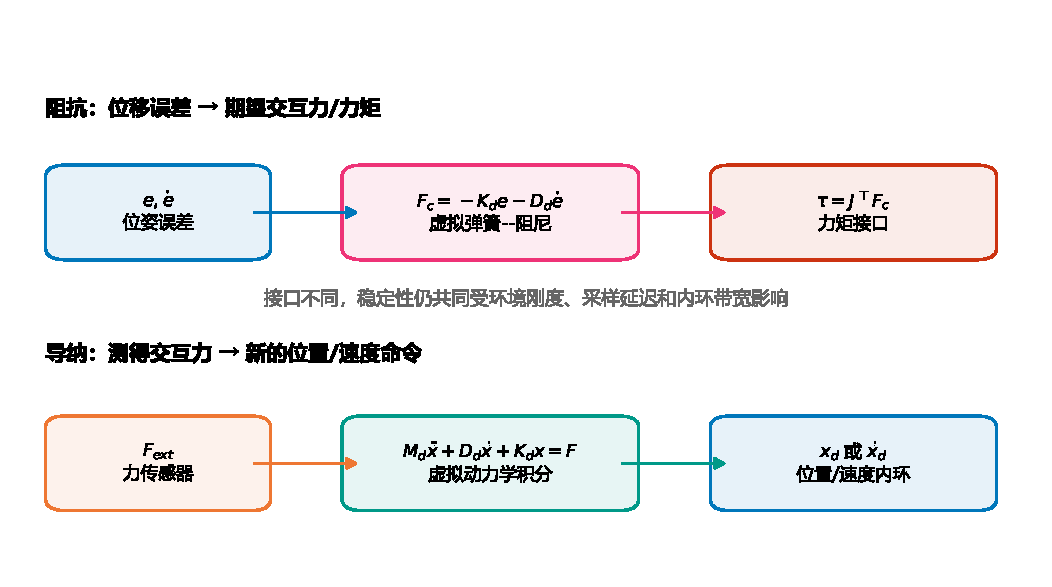
\includegraphics[width=\textwidth]{v0.3-06-阻抗与导纳接口.pdf}
\caption{阻抗与导纳的信号方向和执行器接口。作者依据经典力控制分类绘制\cite{hogan1985impedance,deschutter1997force}。}
\label{fig:impedance-admittance-interface}
\end{figure}

图\ref{fig:impedance-admittance-interface}中的差别决定代码落点。阻抗外环从位置/速度误差计算期望交互力或关节力矩，依赖可控力矩接口；导纳外环从测得外力积分出新的位置/速度命令，可包在厂商位置伺服器之外。后者并不天然更稳定：力传感噪声会被积分，位置内环延迟又会改变虚拟质量、阻尼和环境刚度组成的闭环极点。

\subsection{一维参数算例}

设期望接触方向的虚拟质量 $m_d=2\ \mathrm{kg}$、刚度 $k_d=800\ \mathrm{N/m}$。临界阻尼为 $d_d=2\sqrt{m_dk_d}=80\ \mathrm{N\,s/m}$，固有频率 $\omega_n=\sqrt{k_d/m_d}=20\ \mathrm{rad/s}$。若环境位置误差为 $2\ \mathrm{mm}$，静态弹簧力约为 $1.6\ \mathrm{N}$；若标定误差增至 $10\ \mathrm{mm}$，则为 $8\ \mathrm{N}$。控制律没有改变，但几何误差把交互力放大了五倍。这就是为什么接触控制章节必须同时讨论标定、阈值和回退。

\section{官方实现导读：方程如何落到实时回调}

libfranka 0.15.0 的官方示例在 1 个实时回调中读取科氏项、末端雅可比和关节速度，构造弹簧--阻尼任务力矩，并把科氏补偿相加\cite{libfranka015}。以下片段保留其关键计算，省略连接、姿态误差和异常处理：

\begin{lstlisting}[language=C++,caption={libfranka 0.15.0 笛卡尔阻抗示例的关键力矩计算（Apache-2.0）}]
auto coriolis_array = model.coriolis(robot_state);
auto jacobian_array = model.zeroJacobian(
    franka::Frame::kEndEffector, robot_state);
Eigen::Map<const Eigen::Matrix<double, 7, 1>>
    coriolis(coriolis_array.data());
Eigen::Map<const Eigen::Matrix<double, 6, 7>>
    jacobian(jacobian_array.data());
Eigen::Map<const Eigen::Matrix<double, 7, 1>>
    dq(robot_state.dq.data());
tau_task = jacobian.transpose()
         * (-stiffness * error - damping * (jacobian * dq));
tau_d = tau_task + coriolis;
\end{lstlisting}
\sourceanchor{仓库 \texttt{frankarobotics/libfranka}；tag \texttt{0.15.0}；文件 \texttt{examples/cartesian\_impedance\_control.cpp}；许可证 Apache-2.0；符号 \texttt{impedance\_control\_callback}。}

代码与式\eqref{eq:desired-impedance}之间存在三个值得检查的差异。第一，示例明确“不做惯量整形”，所以 $M_d$ 不是任意指定的常数矩阵；实际闭环惯量随构型变化。第二，示例的旋转误差由四元数构造，不能把欧氏角度误差原样复制。第三，官方文档警告该示例把碰撞阈值设得较高，并要求操作者握住急停。示例能解释算法，不等于通过生产安全验证。

\section{完整案例：带搜索与回退的柔顺插装}

考虑圆柱销插入孔。已知末端标称孔位 $\hat x_h$，但横向误差可能达到 $\pm2\ \mathrm{mm}$；六维力/力矩传感器提供 $w=[f_x,f_y,f_z,m_x,m_y,m_z]$。任务不是“沿 $z$ 轴下降”，而是一个带观测判据的状态机：

\begin{figure}[H]
\centering
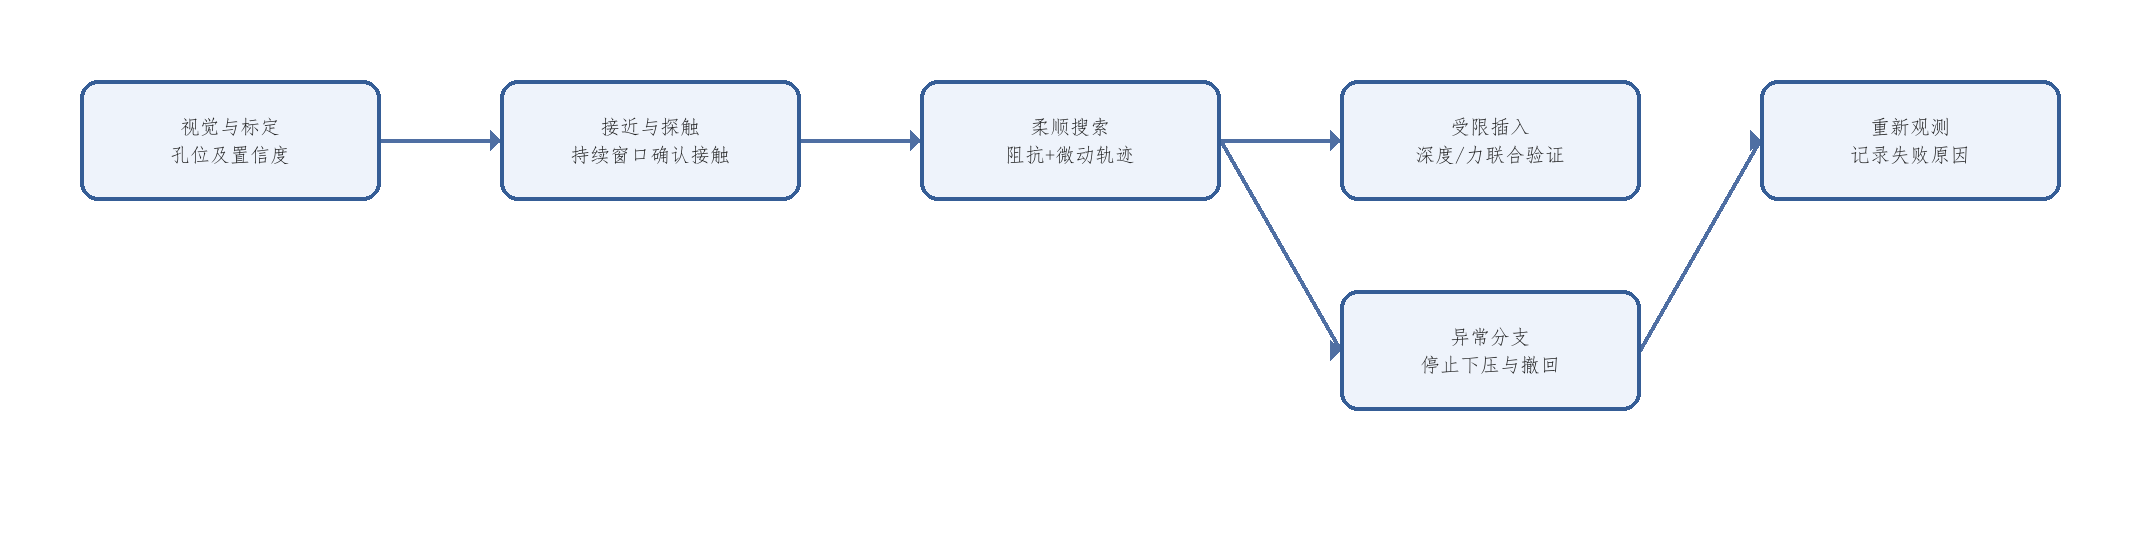
\includegraphics[width=\textwidth]{v0.3-06-柔顺插装闭环.png}
\caption{柔顺插装的观测、控制与异常恢复链。作者自绘；概念依据为阻抗/力控制文献\cite{hogan1985impedance,deschutter1997force}，不复制论文原图。}
\label{fig:compliant-insertion-loop}
\end{figure}

\begin{enumerate}
  \item \textbf{接近：}在自由空间移动到孔上方，限制速度和动能；检查视觉置信度、工具标定版本和工件是否到位。
  \item \textbf{探触：}沿 $-z$ 低速移动。当 $f_z>f_{contact}$ 持续 $N$ 个采样周期时确认接触，避免单点噪声触发。
  \item \textbf{搜索：}保持法向期望力或低法向刚度，在 $xy$ 平面执行螺旋/栅格微动；横向力和力矩用于判断卡边。
  \item \textbf{插入：}检测到 $z$ 位移增加且横向力下降后，切换到较高横向刚度和受限轴向速度。
  \item \textbf{验证：}以深度、末端残余力和工件存在信号共同判定成功；单一位置阈值可能把工件变形误判为到位。
  \item \textbf{回退：}若 $\|f_{xy}\|>f_{jam}$、$|m_{xy}|>m_{jam}$ 或搜索超时，立即停止下压，沿已知安全方向撤回，重新观测孔位；重复次数超过上限则转人工。
\end{enumerate}

\begin{lstlisting}[language=Python,caption={教学伪代码：插装状态机；非任何厂商源码}]
while not terminal:
    wrench = low_pass(read_wrench())
    if state == APPROACH:
        command_pose(pre_insert)
    elif state == TOUCH and persistent(wrench.fz > f_contact, N):
        state = SEARCH
    elif state == SEARCH:
        command_impedance(spiral_xy(), vz=-v_probe, K=K_search)
        if insertion_signature(depth, wrench): state = INSERT
        if jam(wrench) or timeout(): state = RETRACT
    elif state == RETRACT:
        stop_downward_motion(); retract(); reacquire_hole()
\end{lstlisting}

这段伪代码故意把控制命令与判据分开。$f_{contact}$、$f_{jam}$ 和滤波窗口不能凭经验永久写死：它们需要由传感器噪声、正常接触分布、工件公差和允许风险共同标定。部署日志至少应保存原始/滤波力、位姿、状态转换原因、控制器参数和失败图像，否则失败样本无法回流到几何估计或策略训练。

\section{知识小结与综述判断}

\textbf{知识小结。}关节空间动力学把执行器力矩、惯性、科氏/离心、重力和接触广义力置于同一方程；单边接触由间隙、法向力和互补条件描述，摩擦锥区分粘着与滑动；任务空间惯量说明末端方向上的动态响应随构型变化；阻抗与导纳控制分别规定运动--力关系及力到运动的外环映射。柔顺插装需要状态机、阈值和恢复链，不能只给出一条控制方程。

\authorjudgement{经典阻抗和操作空间理论仍是接触操作的主干，不是等待被 VLA 淘汰的“传统模块”。学习策略最有价值的切入点通常是难以建模的搜索轨迹、接触状态估计和参数调节；安全力限、实时内环、急停与确定性回退仍应由可验证的控制层承担。若一项工作只报告成功率而不报告接触力、超时、卡死和人工恢复，它不足以证明接触操作能力。}

\chapter{代表性 VLA 的设计比较}
\label{chap:vla-design-comparison}

\section{问题设定：比较的是闭环策略，不是模型名气}

视觉--语言--动作模型（Vision--Language--Action, VLA）把观测 $o_t$、语言条件 $l$、本体状态 $s_t$ 映射为动作或动作块。统一写成
\begin{equation}
a_{t:t+H-1}\sim\pi_\theta(\,\cdot\mid o_{t-k:t},s_{t-k:t},l\,),
\label{eq:vla-policy}
\end{equation}
其中 $H$ 是预测动作块长度，$k$ 是历史窗口。式\eqref{eq:vla-policy}隐藏了会直接改变系统行为的六个选择：动作坐标系、动作分布族、时间离散、解码次数、执行多少步后重规划，以及低层控制器如何跟踪动作。只比较参数量或论文成功率会把这些差异抹平。

RT-1 证明了大规模多任务真机数据与高容量序列模型可以形成可扩展的机器人策略\cite{brohan2022rt1}；RT-2 进一步把动作表示并入 VLM 的 token 输出空间\cite{brohan2023rt2}。但“把动作写成 token”只是一个设计分支。Diffusion Policy 和 Octo 直接建模连续动作分布\cite{chi2023diffusion,octo2024}，$\pi_0$ 使用 flow matching\cite{black2024pi0}，GR00T N1 则把视觉语言推理与 diffusion transformer 动作模块组织成双系统\cite{nvidia2025groot}。

\section{动作表示的四种基本路线}

\begingroup
\hbadness=10000
\begin{figure}[H]
\centering
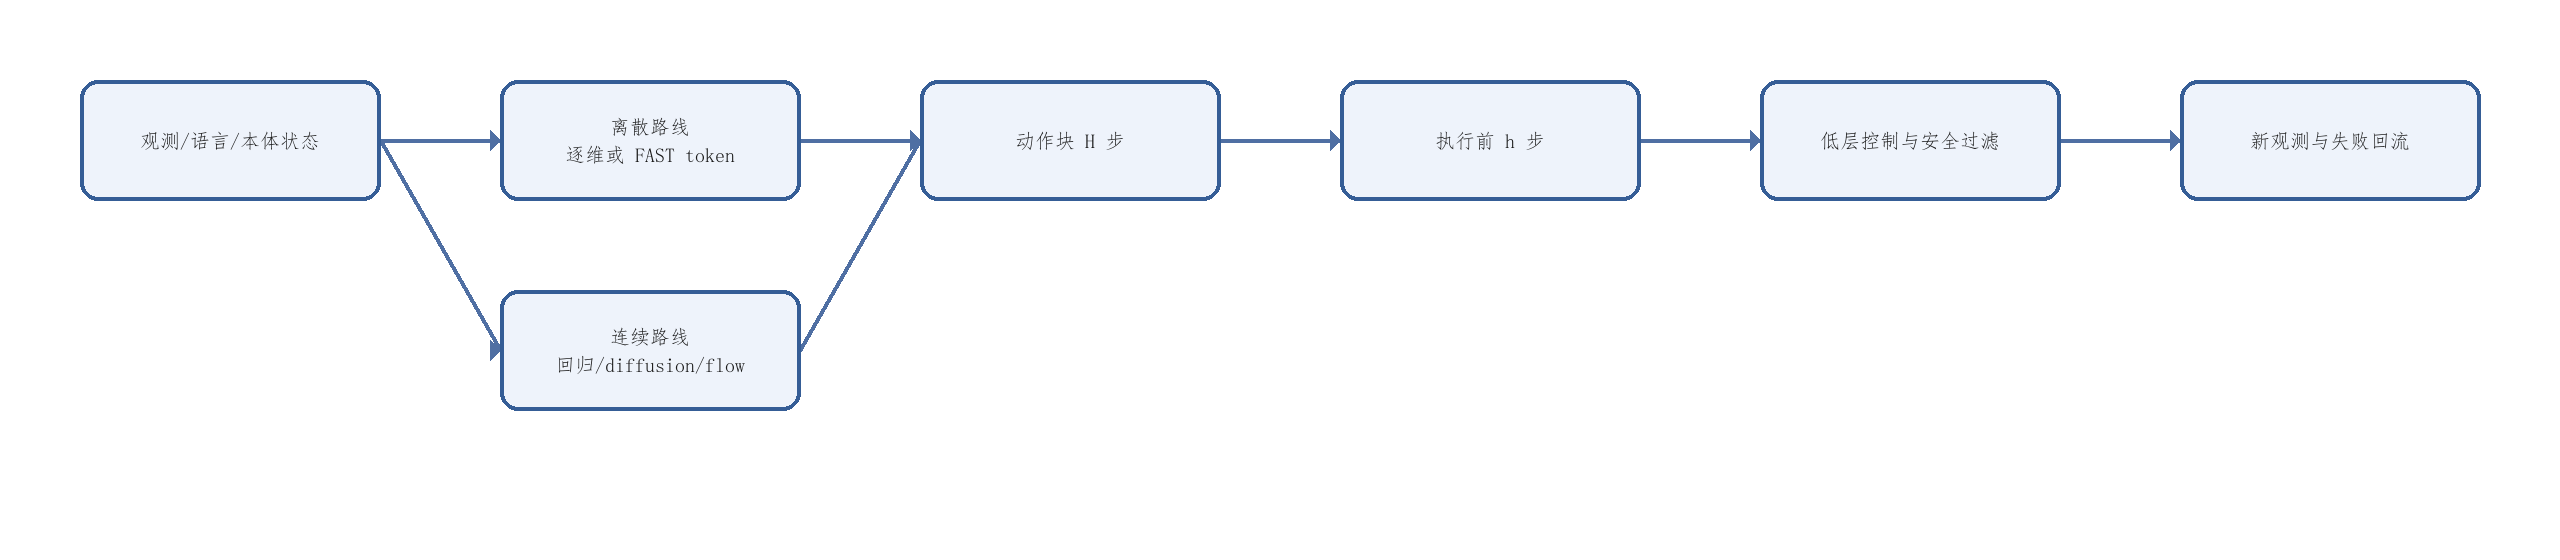
\includegraphics[width=\textwidth]{v0.3-23-VLA动作表示坐标.png}
\caption{动作表示、动作块与低层闭环之间的关系。作者依据 RT-2、Diffusion Policy、FAST 与 $\pi_0$ 的公开方法改绘\cite{brohan2023rt2,chi2023diffusion,pertsch2025fast,black2024pi0}。}
\label{fig:vla-action-design-space}
\end{figure}

\subsection{逐维回归：快，但容易把多峰行为平均掉}

若策略输出高斯均值，常用目标为
\begin{equation}
\mathcal L_{\mathrm{MSE}}=\mathbb E\|a_t-f_\theta(o_t,s_t,l)\|_2^2.
\end{equation}
它只需一次前向传播，适合低延迟控制；但当绕障可以向左也可以向右、抓取存在多个等价姿态时，条件均值可能落在两种可行动作之间。Mixture Density、离散 latent 或生成式动作头的目的，不是“让模型更大”，而是恢复条件动作分布的多峰结构。

这个结论可以直接从损失函数得到。对固定条件 $c=(o_t,s_t,l)$，把标量输出记为 $y$，则
\begin{equation}
\frac{\partial}{\partial y}\,\mathbb E[(a-y)^2\mid c]
=2\left(y-\mathbb E[a\mid c]\right),
\end{equation}
所以平方误差的最优点估计必为条件均值 $y^*=\mathbb E[a\mid c]$。若演示者以相同概率选择 $a=-1$ 和 $a=+1$，两种动作都可行，回归器却会输出 $0$。在绕障任务中，$0$ 可能恰好指向障碍物；这不是训练不足，而是“单峰点估计”与“多峰决策”之间的结构冲突。

\begin{figure}[H]
\centering
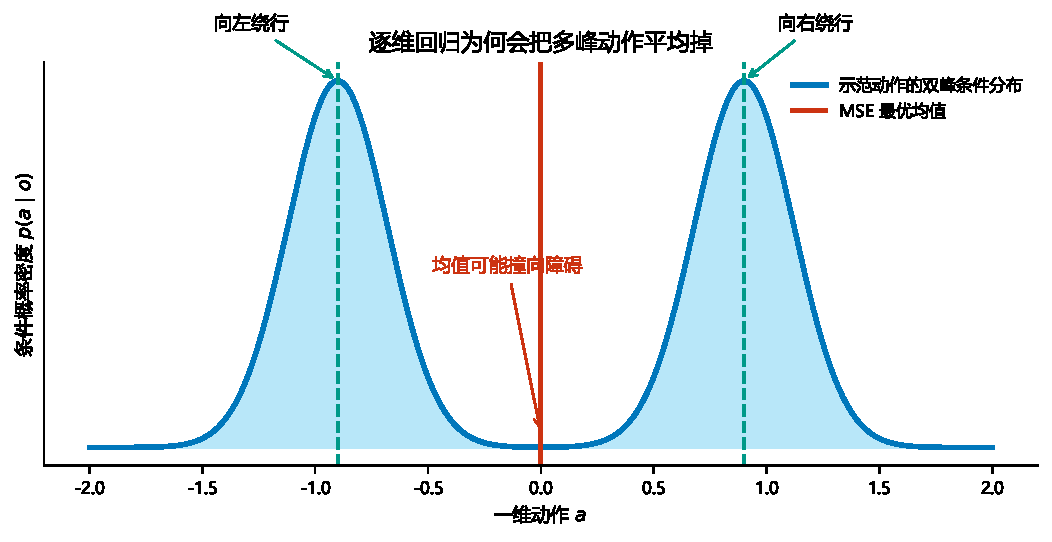
\includegraphics[width=0.92\textwidth]{v0.3-23-回归多峰平均.pdf}
\caption{平方误差把双峰动作分布压成条件均值的教学示意。曲线为作者生成的合成分布，不是论文实验结果。}
\label{fig:regression-mode-averaging}
\end{figure}

\subsection{离散动作 token：复用语言模型目标，但量化不是免费的}

将归一化动作 $a^{(j)}\in[-1,1]$ 均匀量化为 $B$ 个区间，
\begin{equation}
z^{(j)}=\operatorname{clip}\!\left(\left\lfloor\frac{a^{(j)}+1}{2}B\right\rfloor,0,B-1\right),
\qquad
\hat a^{(j)}=-1+\frac{2z^{(j)}+1}{B}.
\label{eq:uniform-action-token}
\end{equation}
于是训练可复用自回归交叉熵。RT-1 采用离散动作 token；RT-2 和 OpenVLA 让动作 token 与语言 token 共处输出词表\cite{brohan2022rt1,brohan2023rt2,kim2024openvla}。优势是训练基础设施成熟、输出概率可解释；代价是每个维度/时刻都占 token，量化误差与序列长度随控制维度和频率上升。

令分箱宽度 $\Delta=2/B$。若用箱中心解码且动作未被裁剪，单维最大量化误差为 $\Delta/2=1/B$；$B=256$ 时归一化误差上界约为 $0.0039$。这个数字必须乘回各维物理量程：同一归一化误差，对 $\pm1$ rad 的关节角与 $\pm0.1$ m 的位移不是同一控制误差。动作块含 $H$ 个时刻、每时刻有 $D$ 个独立离散维度时，朴素自回归序列长为 $DH$；例如 $D=7,H=50$ 就是 350 个动作 token。量化精度、解码延迟和上下文占用因此构成三方权衡。

\begin{figure}[H]
\centering
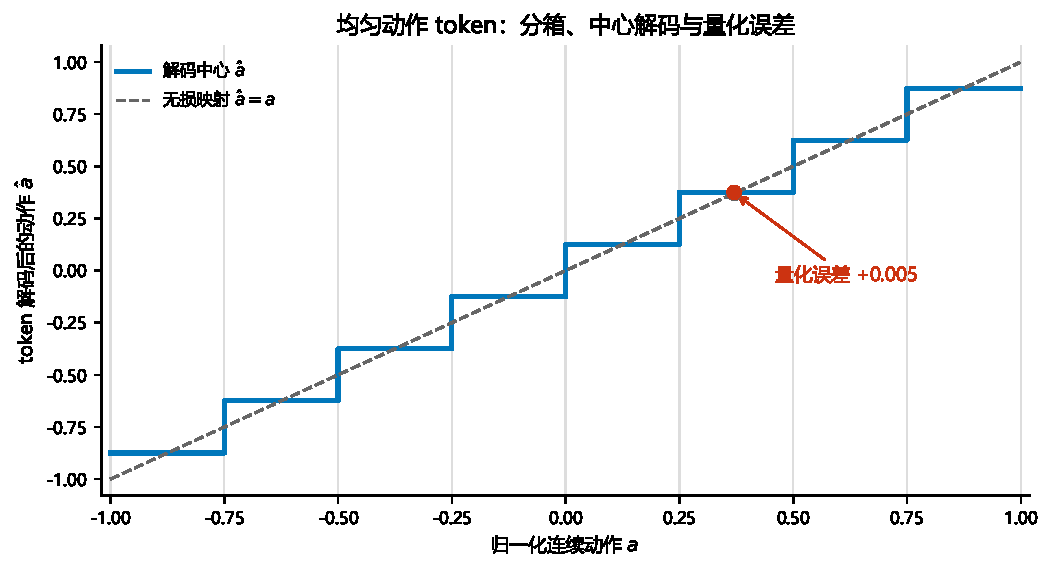
\includegraphics[width=0.94\textwidth]{v0.3-23-动作token量化.pdf}
\caption{均匀动作分箱的阶梯解码与误差。作者依据 OpenVLA 的动作 tokenizer 逻辑绘制\cite{kim2024openvla,openvla2024code}；图中使用 $B=8$ 仅为放大展示量化效应。}
\label{fig:action-token-quantization}
\end{figure}

FAST 指出逐维逐时刻分箱在高频灵巧动作上表现不佳，因而先对动作块做离散余弦变换，再对频域系数编码；FAST+ 在多机器人动作轨迹上学习通用 tokenizer\cite{pertsch2025fast}。这揭示了一个更一般的原则：动作 tokenizer 应利用时间相关性，而不是把每个采样点当作相互独立的“词”。

\subsection{扩散动作：表达多峰分布，以迭代换取计算}

令 $A^0=a_{t:t+H-1}$ 为干净动作块，前向过程加噪得到
\begin{equation}
A^\tau=\sqrt{\bar\alpha_\tau}A^0+\sqrt{1-\bar\alpha_\tau}\epsilon,
\qquad \epsilon\sim\mathcal N(0,I),
\end{equation}
噪声预测目标为
\begin{equation}
\mathcal L_{\mathrm{diff}}=
\mathbb E_{A^0,\tau,\epsilon}
\left\|\epsilon-\epsilon_\theta(A^\tau,\tau,o,s,l)\right\|_2^2.
\label{eq:diffusion-loss}
\end{equation}
推理从高斯噪声开始迭代去噪。Diffusion Policy 把这一过程与视觉条件、时间序列动作块和滚动时域执行结合，在其 12 项任务/4 组 benchmark 的实验集合中报告相对既有方法平均提升 46.9\%\cite{chi2023diffusion}。该数值不能直接与 OpenVLA 或 Gemini Robotics 的不同任务成功率相减。

训练和推理方向不能混为一谈。训练时先从数据集取干净动作 $A^0$，随机采样噪声等级 $\tau$ 和高斯噪声 $\epsilon$，只需构造一个带噪样本并回归噪声；推理时没有 $A^0$，必须从随机噪声出发，按噪声日程多次调用网络。不同随机初值可以收敛到不同动作模式，因此它能保留图\ref{fig:regression-mode-averaging}中被均值回归抹掉的选择。Diffusion Policy 还采用滚动时域：预测一段、执行前若干步、再用新观测重算；原论文 Fig.~3 把这件事与视觉条件去噪网络并列呈现\cite{chi2023diffusion}。

\begin{figure}[H]
\centering
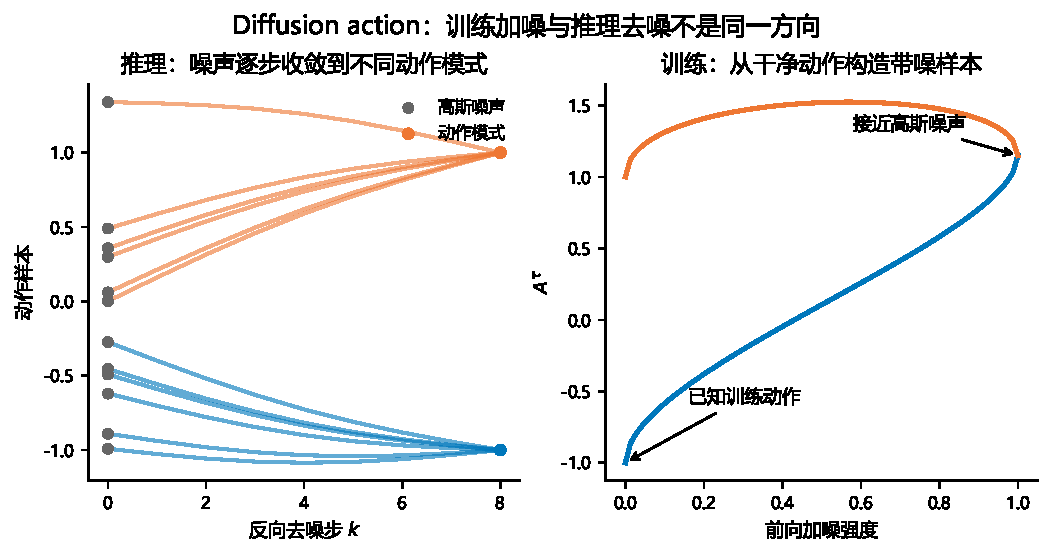
\includegraphics[width=\textwidth]{v0.3-23-扩散动作生成.pdf}
\caption{扩散动作的训练加噪与推理去噪方向。作者根据 Diffusion Policy 的方法与原论文 Fig.~1、Fig.~3 重新组织绘制\cite{chi2023diffusion}，不复制原图像素；轨迹为教学示意。}
\label{fig:diffusion-action-generation}
\end{figure}

Octo 采用 Transformer 主干和 diffusion readout，重点不是单一动作空间上的最高分，而是让不同相机、本体状态、任务条件和动作头以模块化 token group 接入，并在目标域小数据上微调\cite{octo2024}。扩散的工程代价是一次动作块需要多次网络评估；若动作块执行期间不重规划，快速生成并不等于快速闭环。

\subsection{流匹配：学习速度场，仍需数值积分}

取噪声 $A^0\sim\mathcal N(0,I)$、数据动作 $A^1\sim p_{data}$，线性概率路径
\begin{equation}
A^\tau=(1-\tau)A^0+\tau A^1,\qquad
u_\tau=A^1-A^0.
\end{equation}
流匹配训练速度场 $v_\theta$：
\begin{equation}
\mathcal L_{\mathrm{FM}}=
\mathbb E\left\|v_\theta(A^\tau,\tau,o,s,l)-u_\tau\right\|_2^2.
\label{eq:ch23-flow-matching}
\end{equation}
推理时积分 $dA/d\tau=v_\theta(A,\tau,\cdot)$。$\pi_0$ 在预训练 VLM 上接入 flow-matching 动作专家，以连续动作块覆盖单臂、双臂和移动操作平台\cite{black2024pi0}。与扩散相比，流匹配可使用较直接的常微分方程路径，但延迟仍取决于积分步数、主干缓存和硬件，不能由“flow”一词推断为单步控制。

具体地，以 $N$ 步显式 Euler 积分为例，$\Delta\tau=1/N$，
\begin{equation}
A_{i+1}=A_i+\Delta\tau\,v_\theta(A_i,\tau_i,o,s,l),
\qquad i=0,\ldots,N-1.
\label{eq:flow-euler}
\end{equation}
每一步都要在当前动作状态重新估计速度。$\pi_0$ 的公开论文实现以 PaliGemma 视觉语言主干配合约 300M 参数的动作专家，预测 $H=50$ 的动作块，并在所述实验中以 10 个 Euler 步完成积分\cite{black2024pi0}。其块状因果注意力允许视觉语言前缀被缓存，动作专家则在不同积分步更新；因此“10 步”不等于把整个大主干完整运行 10 次，但也绝不是一次前向传播。

\begin{figure}[H]
\centering
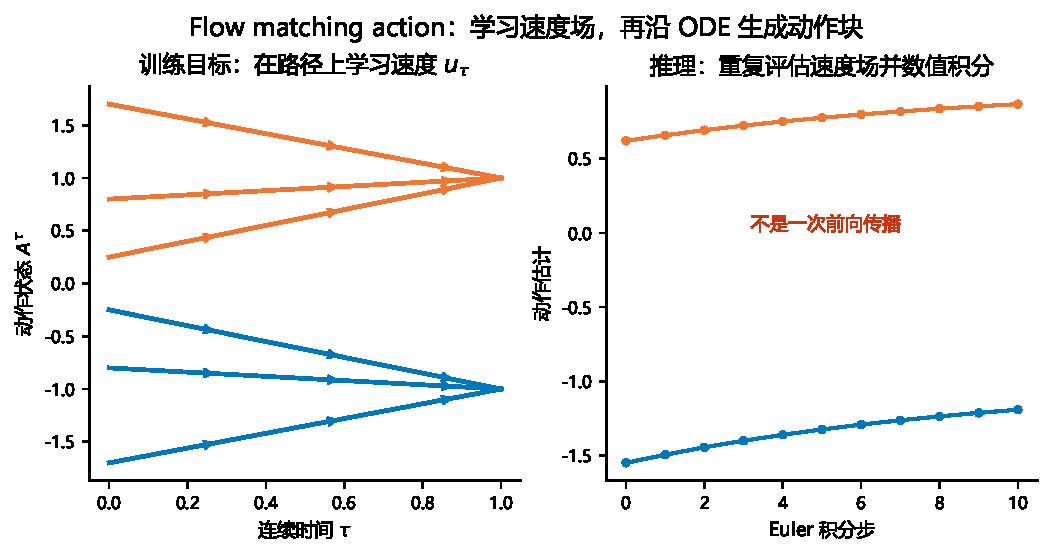
\includegraphics[width=\textwidth]{v0.3-23-流匹配动作生成.pdf}
\caption{流匹配的训练速度场与 Euler 推理。作者依据 $\pi_0$ 的 flow-matching 动作专家改绘\cite{black2024pi0}；路径为二维教学投影。}
\label{fig:flow-matching-action-generation}
\end{figure}

\section{动作块与闭环：$H$ 大不等于长时程智能}

预测 $H$ 步动作块能减少视觉主干调用并让动作在时间上连贯。部署时通常只执行前 $h\le H$ 步，再用新观测重规划。$h=H$ 接近开环动作块，延迟低但对扰动迟钝；$h=1$ 闭环最紧，但计算和通信压力最大。合理选择依赖三个时间尺度：相机/状态更新频率、VLA 推理时间和低层控制周期。

例如 50 Hz 动作数据、$H=50$ 表示 1 秒动作块。若模型用 200 ms 生成一次并执行前 10 步，则重规划周期为 200 ms；若执行全部 50 步，模型虽能提前 800 ms 空闲，却可能在物体被移动后继续执行旧动作。论文若只写“输出 50-step chunk”而不报告 $h$、推理延迟、低层跟踪和观测新鲜度，读者无法判断闭环能力。

\section{主干与动作头如何分工}

PaLM-E 把图像、连续状态估计和文本编码交错输入语言模型，证明具身传感可以进入大型多模态主干，但其代表性机器人任务更多落在具身推理和规划，并不等价于一个高频低层控制策略\cite{driess2023palme}。RT-2 则明确把动作写入 VLM 输出空间，使网页语义预训练与机器人控制共同训练\cite{brohan2023rt2}。这一区分阻止了常见误写：不能因为模型“看见机器人并输出计划”就把它归为直接动作 VLA。

RT-1 的输入端以 EfficientNet 提取图像特征，并用 FiLM 接入语言条件；TokenLearner 压缩视觉 token 后，Transformer 按时间建模并输出离散动作。RT-2 改变的关键并非“再加一层 Transformer”，而是把机器人动作写进 VLM 的文本化输出空间，以网页视觉语言任务与机器人轨迹共同训练。PaLM-E 则把连续传感编码成与文本 token 同维的嵌入插入语言模型，更适合作为“感知信息如何进入具身推理主干”的代表。三者都使用 Transformer，但输入组织、监督目标和控制责任不同。

OpenVLA 组合 DINOv2 与 SigLIP 视觉特征、Llama 2 语言主干和离散动作输出，在 970k 真实机器人示范上训练；论文报告其 7B 模型在指定 29 项任务设置中相对 RT-2-X 的绝对成功率优势，以及相对从头训练 Diffusion Policy 的目标域微调优势\cite{kim2024openvla}。这些结果支持其设计在该评测协议下有效，不支持“7B 普遍优于 55B”这种脱离数据与动作接口的结论。

OpenVLA 中，DINOv2 偏向局部视觉表征，SigLIP 提供视觉--语言对齐特征，两路特征拼接后经投影器送入 Llama 2；动作再由语言模型词表末端的一组 token 自回归产生。于是视觉编码器回答“看到了什么”，投影器解决维度/分布接口，语言主干融合指令与图像上下文，ActionTokenizer 才负责连续控制量的编解码。任何一层冻结或微调，都会改变数据需求与部署代价，不能用“Llama 2 输出动作”一句话概括。

图\ref{fig:openvla-original-architecture}给出原论文的完整接口关系。读图时应沿编号 $1\rightarrow2\rightarrow3$ 追踪：DINOv2 与 SigLIP 分别编码同一图像，特征经 MLP projector 投到语言嵌入空间，再与指令 token 一起进入 Llama 2；输出端的 action de-tokenizer 才把词表 token 还原成七维控制量。原图把“视觉融合”和“动作反量化”画在主干两端，说明 OpenVLA 不是把连续向量直接塞给语言模型，而是依赖两个机器人专用接口夹住通用 VLM 主干。

\begin{figure}[H]
\centering
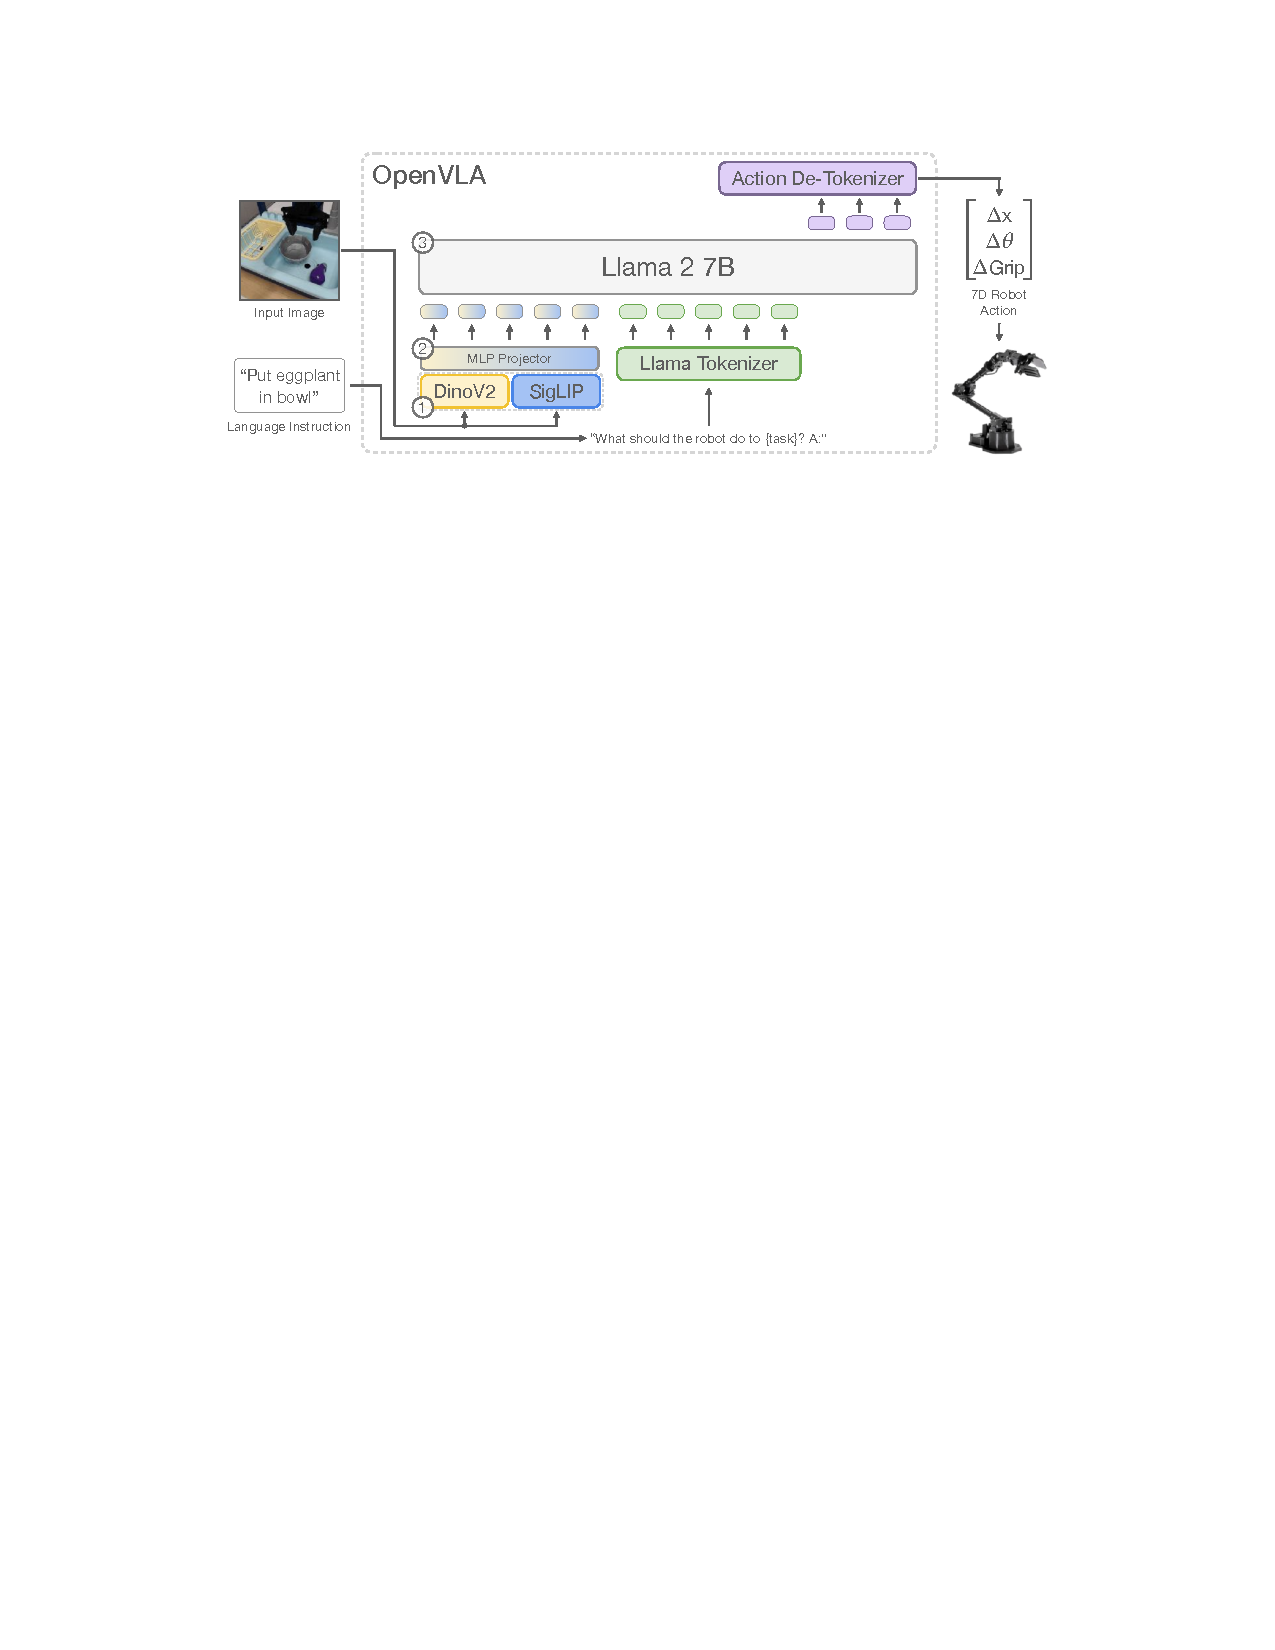
\includegraphics[width=0.96\textwidth]{v0.3-23-OpenVLA-Fig2原图.pdf}
\caption{OpenVLA 模型架构原图。引自 OpenVLA 原论文 Fig.~2（arXiv:2406.09246v3）\cite{kim2024openvla}，CC BY 4.0；从论文第 4 页裁切，仅缩放，未翻译或改绘。}
\label{fig:openvla-original-architecture}
\end{figure}

\subsection{Octo：模块化不是一句“可扩展”}

Octo 的主干输入由若干 \emph{token group} 组成：任务侧可以是语言或目标图像，观测侧可以包含多相机图像和本体状态。各自 tokenizer 先把异构输入变成统一宽度的 token，再由块状注意力掩码规定哪些组能相互读取。主干不直接把最后一个普通 token 当动作，而是加入专用 readout token；readout 汇聚上下文后连接 diffusion action head，产生连续动作块\cite{octo2024}。

这种设计把“共享知识”和“本体接口”分开。迁移到新机器人时，可以增加新的观测 tokenizer 以接收力/力矩或不同相机，也可以替换动作 readout 以适配新的关节维度；共享 Transformer 仍提供从 25 个数据集、约 80 万段轨迹中学到的跨任务表征。它并不意味着零成本跨本体：新增模块仍需目标域数据训练，动作归一化、时间对齐和相机标定也必须重做。

原论文 Fig.~2 还表达了改绘图容易弱化的一点：预训练序列可以反复交错 observation 与 readout，而微调阶段以虚线模块加入新观测和新动作空间。图\ref{fig:octo-original-architecture}保留这一原始视觉编码；图\ref{fig:octo-modular-architecture}则将其重排成中文模块图，便于逐步解释 tokenizer、主干、readout 和动作头的职责。两图承担不同任务，不作为重复插图计数。

\begin{figure}[H]
\centering
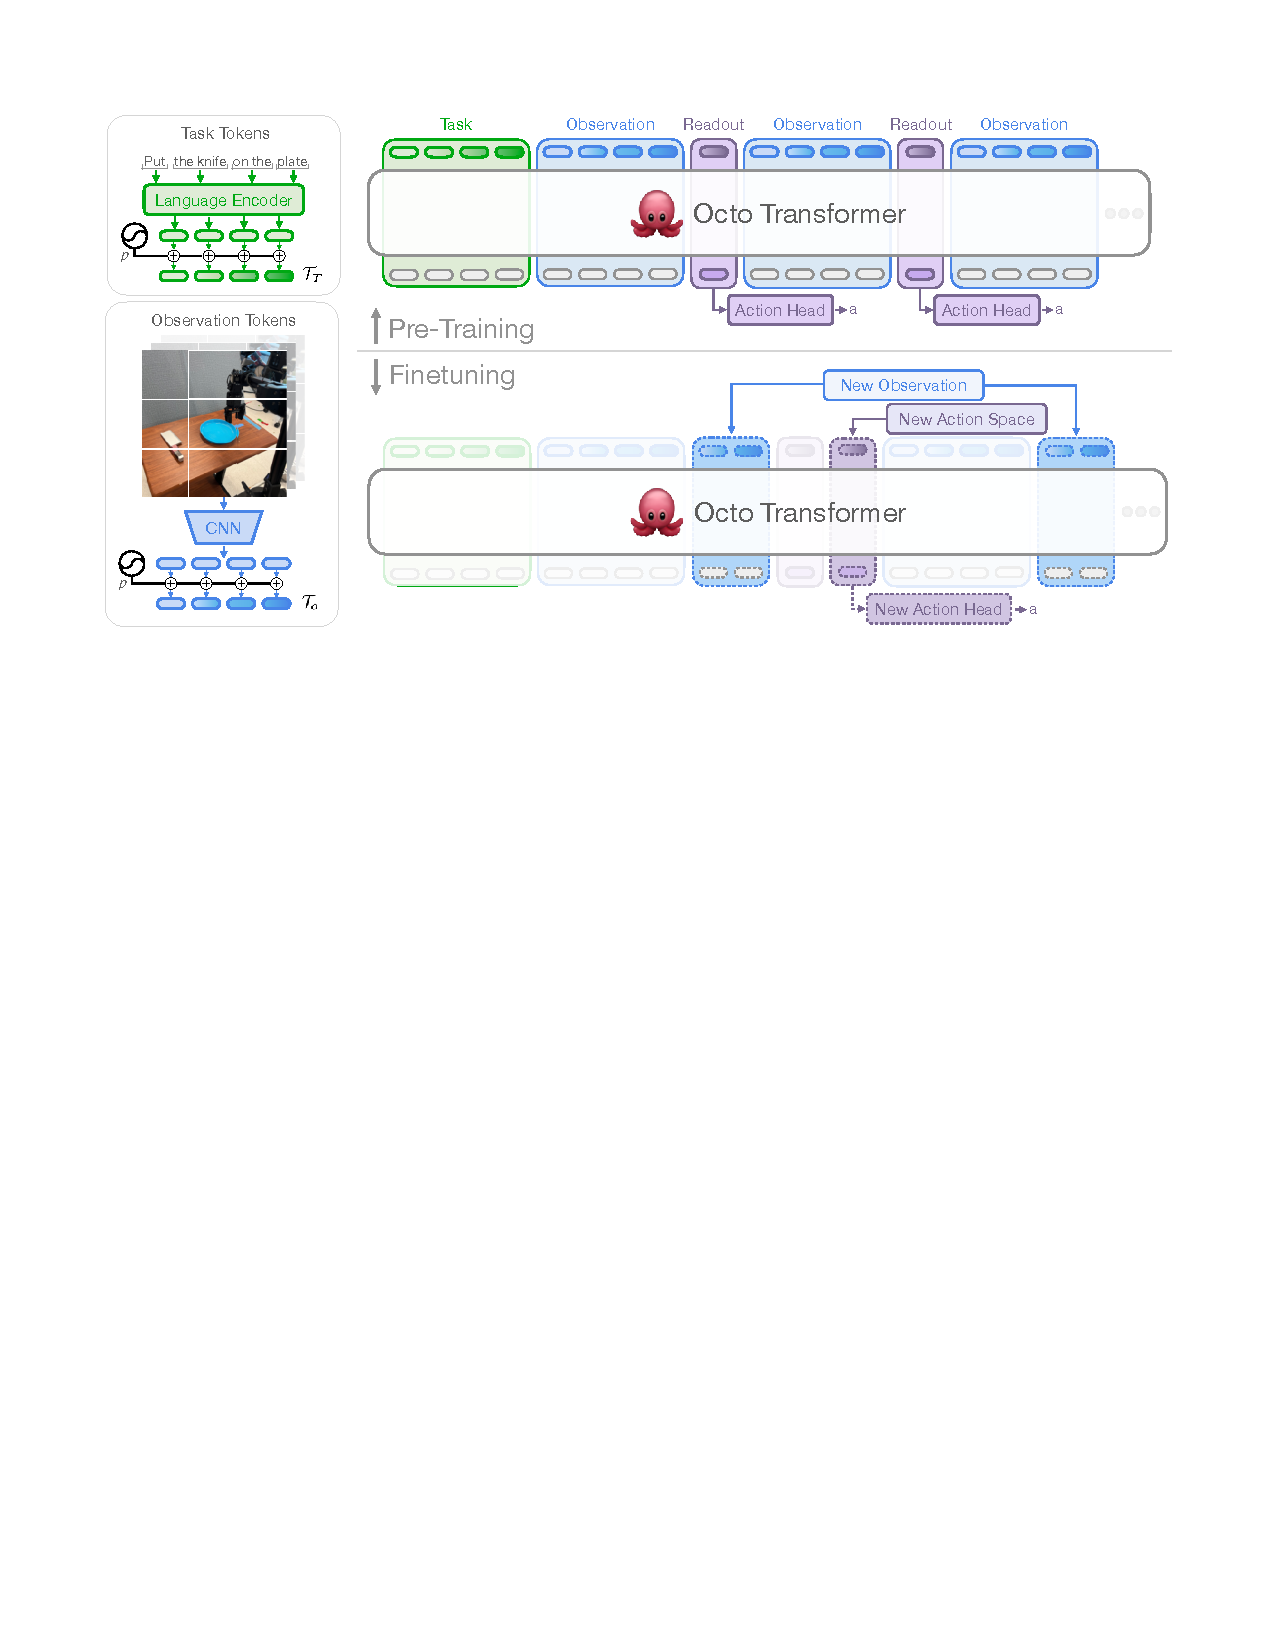
\includegraphics[width=\textwidth]{v0.3-23-Octo-Fig2原图.pdf}
\caption{Octo 模型架构原图。引自 Octo 原论文 Fig.~2（arXiv:2405.12213v2）\cite{octo2024}，CC BY 4.0；从论文第 3 页裁切，仅缩放，未翻译或改绘。}
\label{fig:octo-original-architecture}
\end{figure}
\endgroup

\begin{figure}[H]
\centering
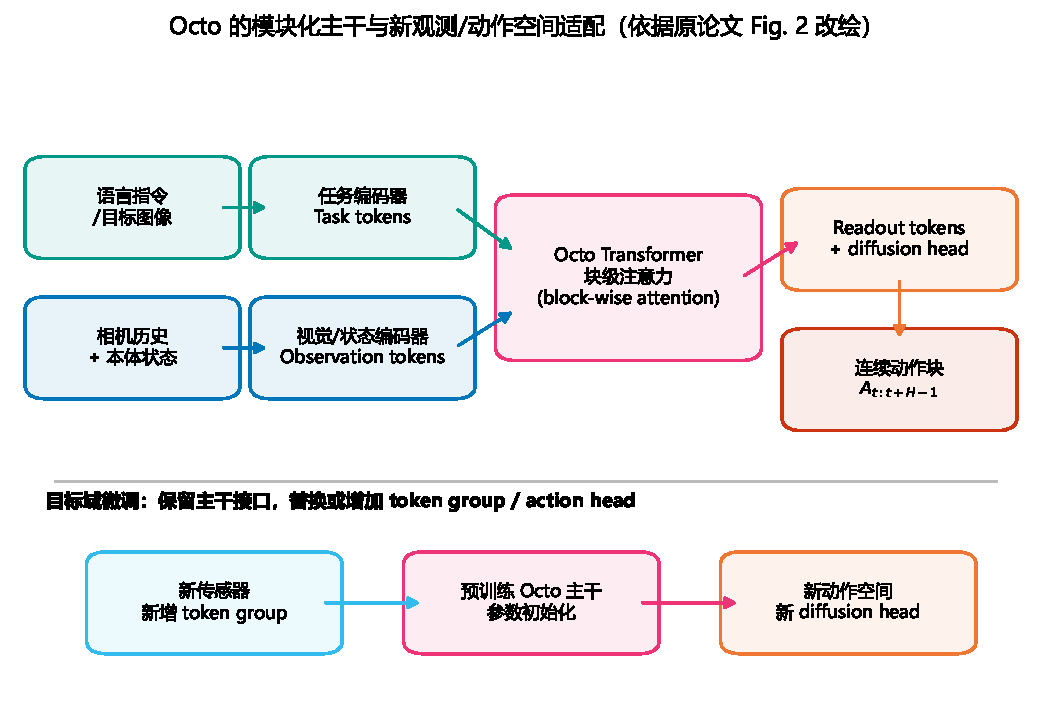
\includegraphics[width=\textwidth]{v0.3-23-Octo模块化架构.pdf}
\caption{Octo 的模块化输入、Transformer 主干、readout 与动作头，以及目标域新增接口。作者依据 Octo 原论文 Fig.~2 改绘\cite{octo2024}，不复制原图像素。}
\label{fig:octo-modular-architecture}
\end{figure}

GR00T N1 把 VLM System 2 与 diffusion transformer System 1 紧耦合并端到端训练，数据混合真实轨迹、人类视频和合成样本\cite{nvidia2025groot}。Gemini Robotics 报告直接控制 VLA；同一技术报告另设 Gemini Robotics-ER，负责空间/时间理解、指向、轨迹与抓取预测等具身推理能力\cite{gemini2025robotics}。二者都提供重要系统证据，但完整训练代码、数据和权重并未公开到足以复现论文主张的程度，开源程度必须与论文新颖性分开评价。

\begingroup
\hbadness=10000
\begin{table}[H]
\centering
\caption{代表性路线的统一设计比较；结果数值因任务与协议不同，不作横向排行榜}
\label{tab:vla-design}
\scriptsize
\begin{tabularx}{\textwidth}{p{0.105\textwidth}p{0.14\textwidth}p{0.13\textwidth}p{0.13\textwidth}p{0.14\textwidth}Y}
\toprule
路线 & 主干/融合 & 动作表示 & 时序与闭环 & 开放证据 & 主要适用条件与限制\\
\midrule
RT-1 & EfficientNet/\allowbreak FiLM、TokenLearner、Transformer & 逐维离散 token & 短历史、实时逐步策略 & 论文与部分官方代码 & 单平台大规模多任务；语义主干不来自通用 VLM\\
PaLM-E & 传感编码与文本 token 交错进 LLM & 以语言/规划输出为主 & 高层推理接口 & 论文，模型闭源 & 不能直接当作低层 VLA 基线\\
RT-2 & VLM 与机器人数据共同训练 & 动作作为文本 token & VLA 直接控制 & 论文，主模型闭源 & 语义迁移强；量化、解码与闭环细节受实现约束\\
Diffusion Policy & 视觉编码器+条件去噪网络 & 连续 diffusion chunk & receding horizon & 论文和官方代码 & 多峰连续动作；多步去噪增加延迟\\
Octo & 模块化 Transformer & diffusion readout & chunk+目标域微调 & 论文、权重、代码 & 新观测/动作空间适配；规模小于大 VLM 路线\\
OpenVLA & DINOv2+\allowbreak SigLIP+\allowbreak Llama 2 & 256-bin 离散 token & 自回归动作输出 & 论文、权重、MIT 代码 & 易复用语言模型栈；高频动作 token 长度和量化受限\\
$\pi_0$ & 预训练 VLM+动作专家 & flow-matching chunk & 数值积分后滚动执行 & 论文、部分权重与 Apache-2.0 代码 & 灵巧连续动作；推理步数和跨本体适配仍需工程验证\\
GR00T N1 & VLM System 2 + DiT System 1 & diffusion action & 双系统端到端 & 报告与开放模型范围 & 人形双臂；开放资产与论文全训练栈并非完全等价\\
Gemini Robotics & Gemini 2.0 基础与机器人专用后训练 & 报告为直接连续控制 & 强调反应式闭环 & 技术报告，核心闭源 & 能力覆盖广；第三方复现与接口细节有限\\
\bottomrule
\end{tabularx}
\end{table}
\endgroup

\section{真实源码导读：OpenVLA 的均匀动作分箱}

OpenVLA 的 \texttt{ActionTokenizer} 清楚展示了式\eqref{eq:uniform-action-token}如何进入代码：先裁剪到动作范围，再逐维分箱，并把分箱编号映射到词表尾部的低频 token\cite{openvla2024code}。

\begin{lstlisting}[language=Python,caption={OpenVLA ActionTokenizer 的关键路径（MIT；为节省篇幅删去类型与批处理分支）}]
self.bins = np.linspace(min_action, max_action, self.n_bins)
self.bin_centers = (self.bins[:-1] + self.bins[1:]) / 2.0

action = np.clip(action, a_min=float(self.min_action),
                 a_max=float(self.max_action))
discretized_action = np.digitize(action, self.bins)
token_ids = self.tokenizer.vocab_size - discretized_action

discretized = self.tokenizer.vocab_size - action_token_ids
discretized = np.clip(discretized - 1, 0,
                      self.bin_centers.shape[0] - 1)
actions = self.bin_centers[discretized]
\end{lstlisting}
\sourceanchor{仓库 \path{openvla/openvla}；许可证 MIT；commit \texttt{c8f03f48\allowbreak af692657\allowbreak d3060c19\allowbreak 588038c7\allowbreak 220e9af9}；文件 \path{prismatic/vla/action_tokenizer.py}；符号 \texttt{ActionTokenizer}。代码逻辑已按 2026-07-13 的 \texttt{main} 页面核验；2026-07-14 通过只读远端查询固定当日 \texttt{main} HEAD，并使用 immutable permalink。}

代码暴露了三个模型图中不易看见的假设。第一，所有动作维统一裁剪到 $[-1,1]$，因此数据统计和反归一化是控制接口的一部分。第二，分箱边界有 256 个而中心只有 255 个，解码需要边界裁剪；“256 个 action token”不等于 256 个等宽可还原中心。第三，映射占用基础 tokenizer 词表末端 token，动作与语言共享词表是工程约定，不是物理上自然的表示。

\section{如何读实验表：先校准任务，再看数字}

跨论文比较至少检查五项：训练数据是否包含测试机器人；任务是 zero-shot、目标域微调还是从头训练；成功判据和试验次数；动作空间与控制频率；是否允许人工复位、重试或高层规划器。Octo 的官方评测覆盖 9 个真机 setup，并报告新力/力矩观测和新关节动作空间的微调\cite{octo2024}；OpenVLA 的 29 项任务、RT-1 的 700+ 数据采集任务与 Gemini Robotics 的能力演示不是同一统计总体。

因此本章不制作“综合成功率排名”。可以比较的是同一论文内部的受控消融，例如 OpenVLA 的视觉特征组合、Octo 的数据/架构选择、Diffusion Policy 的滚动执行与时间序列设计；跨论文只能比较证据边界和接口属性。对闭源模型，作者视频可以证明某次演示发生过，却不能估计总体成功率或失败分布。

\section{知识小结与综述判断}

\textbf{知识小结。}离散 token 把连续动作转成语言模型可处理的分类目标，但引入量化与序列长度；扩散和流匹配能表达多峰连续动作，却需要迭代去噪或数值积分；action chunk 在时间一致性、推理摊销和闭环反应之间权衡。主干是否具备视觉语言知识、动作头是否承担低层控制、执行后何时重规划，是比模型参数量更有解释力的坐标。

\authorjudgement{VLA 研究的核心竞争并不是“谁把最大的 VLM 接到机器人上”，而是谁能在语义泛化、动作分布表达、闭环频率、跨本体归一化和可复现评测之间形成可部署的组合。当前证据尚不足以宣告离散 token、diffusion 或 flow matching 中任何一种取得普遍胜利。对接触密集任务，VLA 最合理的输出通常是受约束动作块或技能参数，仍由本书动力学与接触章定义的实时控制、安全限幅和恢复状态机执行。}


\backmatter
\chapter{References}
\printbibliography[heading=none]
\end{document}
